% Chapter 2

\chapter{Experimental Model} % Main chapter title
\label{Chapter3}

The first phase of this project was to design and select an appropriate 
experimental model. This was essential to gather the necessary data from the 
tested material. This data will be used to determine the design parameters 
that can help to characterize the material's mechanical behavior. \\

The first experimental model had the purpose of serving as a comparator for the experimental 
model II (see section \ref{section:expmod2}). At the beginning of the project, the desired experimental 
model to be analyzed was the second experimental model, which was developed and designed by Yokohama National 
University (YNU). As this second experimental model was still undergoing some improvements and corrections, a similar 
experiment was designed which could fulfill the same purpose.

The chosen experimental characterization for the inverse finite element method for 
 the identification of material parameters for this project was indentation.
The goal of these experiments was to observe the mechanical behavior of a soft material under 
compression using a rounded indenter. The aim was to determine the material behavior and 
observe the response under an indentation larger than the indenter radius. Additionally, 
by performing the indentation tests, the obtained 
data helped for a more in-depth understanding of the material's mechanical behavior for the chosen 
use cases and the determination of the main assumptions for the material modeling.
The main advantage of indentation is the noninvasive feature, which will mostly 
become useful when a test sample should not be modified, e.g., an organ.\\

For both experimental setups, the specimen, which was tested, was made from a human skin gel.
The human skin gel material was a two-component ultra-soft urethane resin.
Polyurethane is widely used for biomedical applications, e.g., preparation of implants, wound dressings, artificial 
organs, and medical supplies. 

Polyurethane can also be used for simulating organ tissues, as it can be tailored to mimic 
and match the mechanical properties of the desired biological tissues \cite{Wang2012}.  Furthermore, polyurethane can be 
synthesized to have a wide range of stiffness, elasticity, viscoelasticity, and can also be prepared 
with complex shapes for medical research purposes \cite{Joseph2018}. \\

In this chapter, the different experimental models, which were used to evaluate the 
mechanical behavior of the ultra-soft polyurethane, will be 
described. In the first two subsections, will focus on the description and 
procedure of the experimental models, followed by explanation of the indentation test 
types. Consequently, an evaluation and analysis of the results will be provided and the 
main assumptions for the design of the material modeling will be defined. 
%The aim in this section is to provide a clear undertanding of the material's mechanical behavior, 
%and describe the first step for the inverse finite element method approach.
% Polyurethane can be easily processed by using 
%standard manufacturing, like %search reference
%here urethane resin avantages. and that it is expected that the material shows a 
\\ 

%----------------------------------------------------------------------------------

\section{Experimental Model I}
\label{section:expmod1}
    
\subsection*{Description of the Experimental Setup}

The first indentation test configuration was done by adapting a tensile and compression 
testing machine, model LTS - 500 NB from MinebeaMitsumi.Inc (Fig. \ref{fig:firstexperiment}). This 
machine possess a maximum load capacity of \SI{500}{\newton}, and test speeds of
\SIlist[per-mode = symbol]{10;20;30;50;75;100}{\milli \metre \per \minute}. To achieve an 
indentation testing configuration, a pin was attached to the movable crosshead holding grip, 
as shown in Fig \ref{fig:500loadcell}.
The indenter had a rounded head made of stainless steel with a
radius of $r_{i1} = \SI{3}{\milli \m}$ and a length of $l_{i1} = \SI{11}{\milli \m}$.

\begin{figure}%
    \centering
   \subfloat[\centering Indentation test configuration with a \SI{500}{\newton} load cell \label{fig:500loadcell}]{{\includegraphics[width=6.5cm]{Images/Experiment/firstexperimentwithtext.png}}}%
   \qquad
   \subfloat[\centering Indentation test configuration with a \SI{10}{\newton} load cell \label{fig:10loadcell}]{{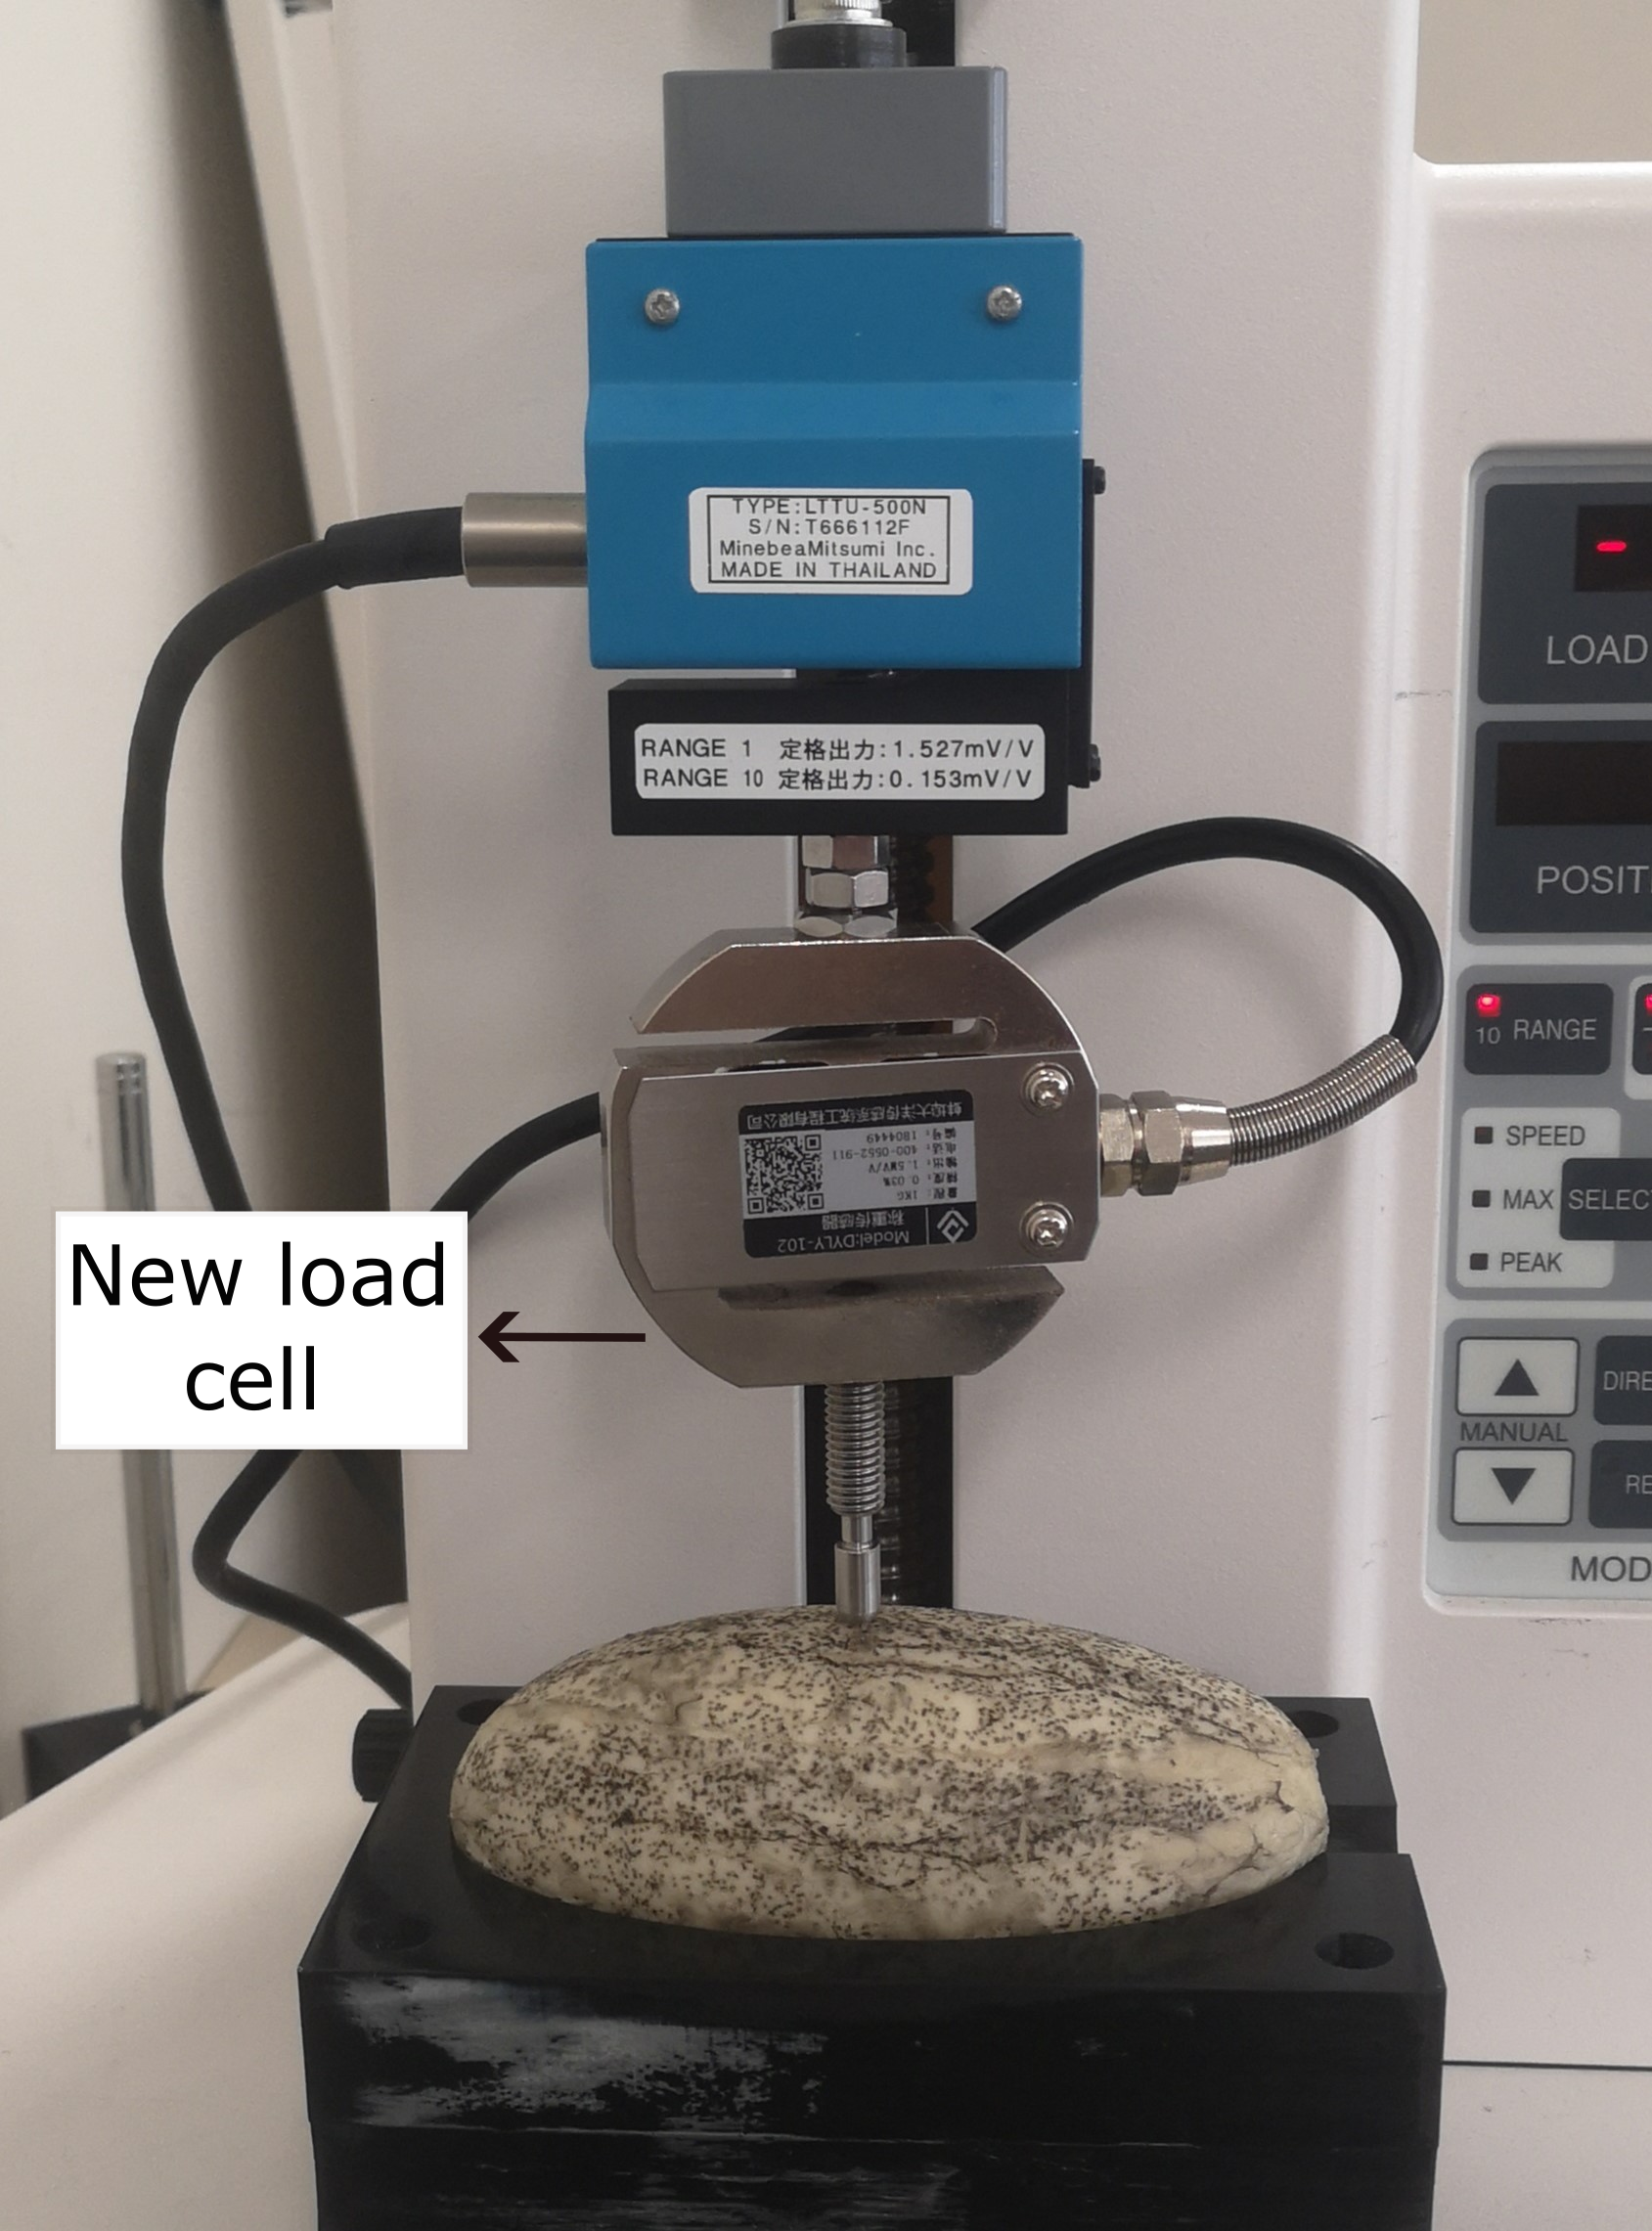
\includegraphics[width=6.5cm]{Images/Experiment/firstexpotherloadwithtext.png}}}%
   \caption{First experimental model: Tensile and compression machine with an indenter with a rounded head. Test Specimen made from ultra-soft polyurethane resin positioned on a fixed platform with a similar shape for constraint.}%
   \label{fig:firstexperiment}%
\end{figure}

The specimen possesses a ellipsoidal form with 
with a minor radius $r_1 = \SI{35}{\milli \m}$ and a major radius $r_2 = \SI{60}{\milli \m}$. 
This specimen geometry is supposed to simulate a kidney with an extracted tumor; therefore,
on the lower part of the specimen a half ellipsoid with a minor radius $r_{l1} = \SI{10}{\milli \m}$ 
and a major radius $r_{l2} = \SI{15}{\milli \m}$ was removed (Fig. \ref{fig:specimenhole}). 
The specimen was prepared by a YNU laboratory member, by 3D printing a mold with the wanted dimensions
 and a ellipsoidal shape, and filling it with liquid resin. 
 Additionally, it was left to cure for around \SI{30} hours. 
Then, the specimen was positioned on a platform fixed to the base, which suited 
the ellipsoidal geometry for properly constraint. 

\begin{figure}%
    \centering
   \subfloat[\centering Specimen dimensions bottom view \label{fig:specimenunder}]{{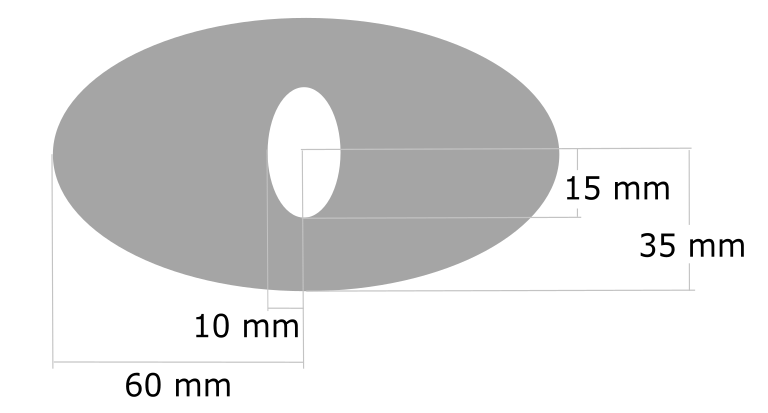
\includegraphics[width=6.5cm]{Images/Experiment/specimenhole.png}}}%
   \qquad
   \subfloat[\centering Specimen side view \label{fig:specimenside}]{{
\includegraphics[width=6.5cm]{Images/Experiment/specimenholeside.png}}}%
   \caption{First experimental model: Specimen dimensions made from ultra-soft polyurethane resin for indentation test.}%
   \label{fig:specimenhole}%
\end{figure}

\subsection*{Procedure for Conducting the Experiment}
For the indentation test after placing the specimen on the platform,
the indenter was positioned slightly on the surface of the point of interest. 
The test was conducted with a room temperature of approximately \SI{22}{\degreeCelsius}
To perform the test the indenter was then lowered onto the surface of the specimen
at a velocity of \SI[per-mode = symbol]{10}{\milli \m\per \minute}.
The indentation depth was controlled by limiting the maximum depth, and the 
test stopped once the inserted depth was reached. The indenter returned to its 
original position after reaching the maximum depth with a rate of 
\SI[per-mode = symbol]{100}{\milli \m\per \minute}. Due to the material properties,
the specimen returned to its original shape.
The result of the indentation test was a load-displacement data,
which was recorded with a sampling rate of \SI{63}{\hertz} using a load 
cell of \SI{\pm 500}{\newton} and a encoder to measure the displacement.

The measurement accuracy according to the specification of the machine, has 
a relative reading error of \SI{1.0}{\percent}. The indentation test 
was repeated five times on the same sample to ensure and observe 
reliability and repeatability. Furthermore, the raw data collected from the test 
was processed and analyzed using Excel.\\

During the initial indentation test using the \SI{500}{\newton} load cell, 
the collected experimental data showed noise that could affect the accuracy 
and reliability of the results. The noise was likely caused by sensitivity 
of the lead cell. The ultra-soft polyurethane material showed force readings, which 
were near the lower limit of the load cell's range, which adding any other external factors, 
results in noisy measurements. To address this issue, a load cell of \SI{10}{\newton}
was installed (Fig. \ref{fig:10loadcell}). This change improved the quality of 
the measurements and reduced the noise in the data. The change to the load cell had some 
implication to the experimental setup, such as removing the holding grip, and designing 
a part which could connect the indenter with the new load cell. In addition to changing 
the load cell, a simple filtering method was used to improve the experimental data. After 
applying the filter, the noise in the data was reduced, resulting in more smoother 
force reaction readings. 

Overall, the applications of the combinations helped to improved the quality and acuracy 
of the data and gave important information about possible measurement errors to 
take into consideration for of the experimental model 
designed by YNU. At last, The filtered data was used for subsequent analysis and 
interpretation for the inverse finite element method approach for the material parameter 
identification.

%iii.	Analysis of different platforms? maybe dont because not enough fotos or info

%----------------------------------------------------------------------------------
\section{Experimental Model II}
\label{section:expmod2}

The second experimental model was developed and designed by Yuta Mori, a 
member of the Yamada Laboratory from the Mechanical Engineering department of 
 Yokohama National University. 
The main aim for this experimental method was to be able to identify the physical 
properties of organs in a state that closely resembles the in vivo environment.
Additionally, this model seeked two achieve two objectives: firstly, to develop a 
loading system to acquire the data required for an inverse analysis, and secondly, 
to establish a measurement process in case of a total nephrectomy \cite{Mori2022}. 

%evtl. speak about ehical use of the experimental model : To ensure the ethical use of the experimental model and data provided by the other master student, I obtained permission from them to use their data in my research. Additionally, I made sure that any ethical considerations related to the data, such as informed consent from participants or privacy concerns, 
%had been appropriately addressed in the original study. As an extra precaution, I also ensured that any identifiable information about the participants had been removed from the data provided by the other master student before incorporating it into my own research. By taking these steps, I ensured that the data was used in a responsible and ethical manner, and that the original research was respected and properly attributed

The resulting data from the experimental model served for the basis of the material 
parameter identification for the inverse finite element method approach.
The processed data obtained from this experimental model assisted in the calibration 
and assessment of the design parameters was employ in the validation for the 
computational model. 

\subsection*{Description and Procedure of the Experimental Setup}
%This article discusses the development of a method to identify the mechanical properties of organs after extraction. 
%The study aims to identify the physical properties of organs immediately after removal to simulate in vivo environments. 
%The study constructs a loading system to acquire data for inverse analysis and establish a measurement process to conduct
% multi-point loading experiments and simultaneously measure the indentation, reaction force, and overall deformation. 
% The study uses a 6-axis force sensor, a laser displacement transducer, and 3D cameras to measure reaction forces, 
% organ deformation, and organ shape. The experimental results show that the method can measure organ mechanical 
% properties and provide data for simulators.

In this experimental model the indentation loading system, which gathers data of the indentation 
depth, reaction force and overall deformation. 
The experimental device consists of an 6-axis force sensor, a laser displacement transducer,
 and 3D cameras placed in four directions to obtain the point cloud data based on the 
 coordinate system of each camera. Fig.\ref{fig:secondexperiment} shows the overall setup of the 
 experiment. For our project, the 6-axis force sensor and the laser displacement were mainly used.
The loading system is operated by specifiying de movement of the loading rod in advance, and the 
indentation is performed in the direction normal to the contact surface to prevent slippage (Fig. \ref{fig:loadingdiag}).\\


 \begin{figure}%
    \centering
   \subfloat[\centering Indentation test configuration front view \label{fig:frontexp2}]{{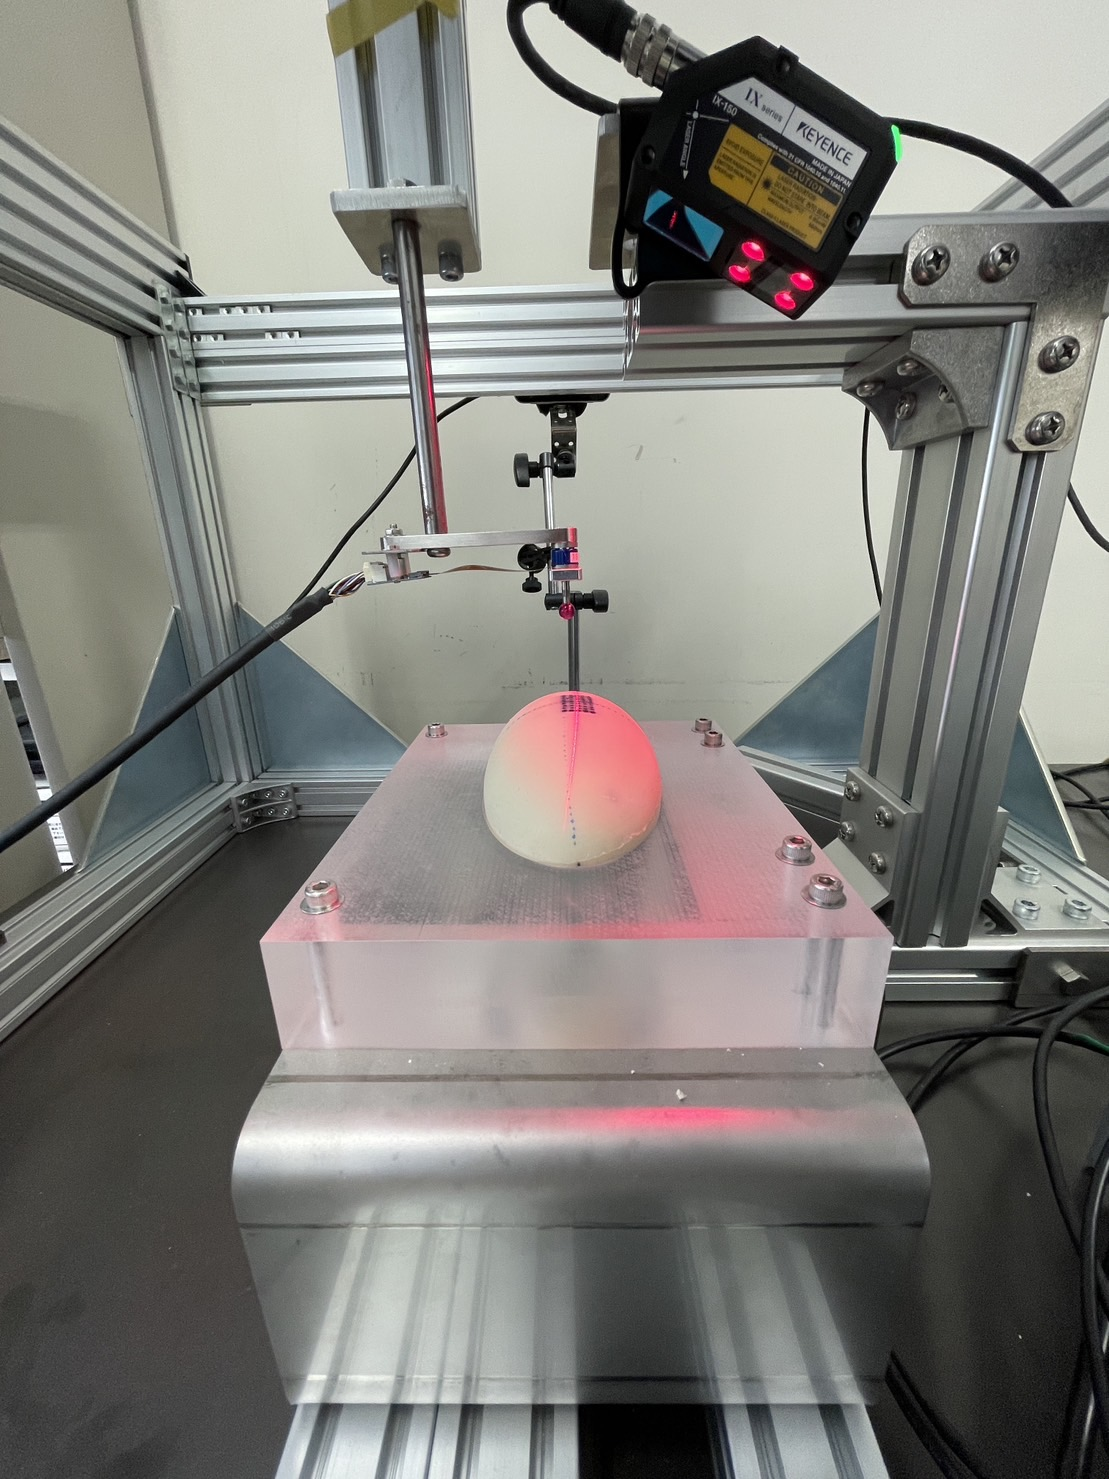
\includegraphics[width=6.5cm]{Images/Experiment/secondexp1}}}%
   \qquad
   \subfloat[\centering Indentation test configuration top view \label{fig:topexp2}]{{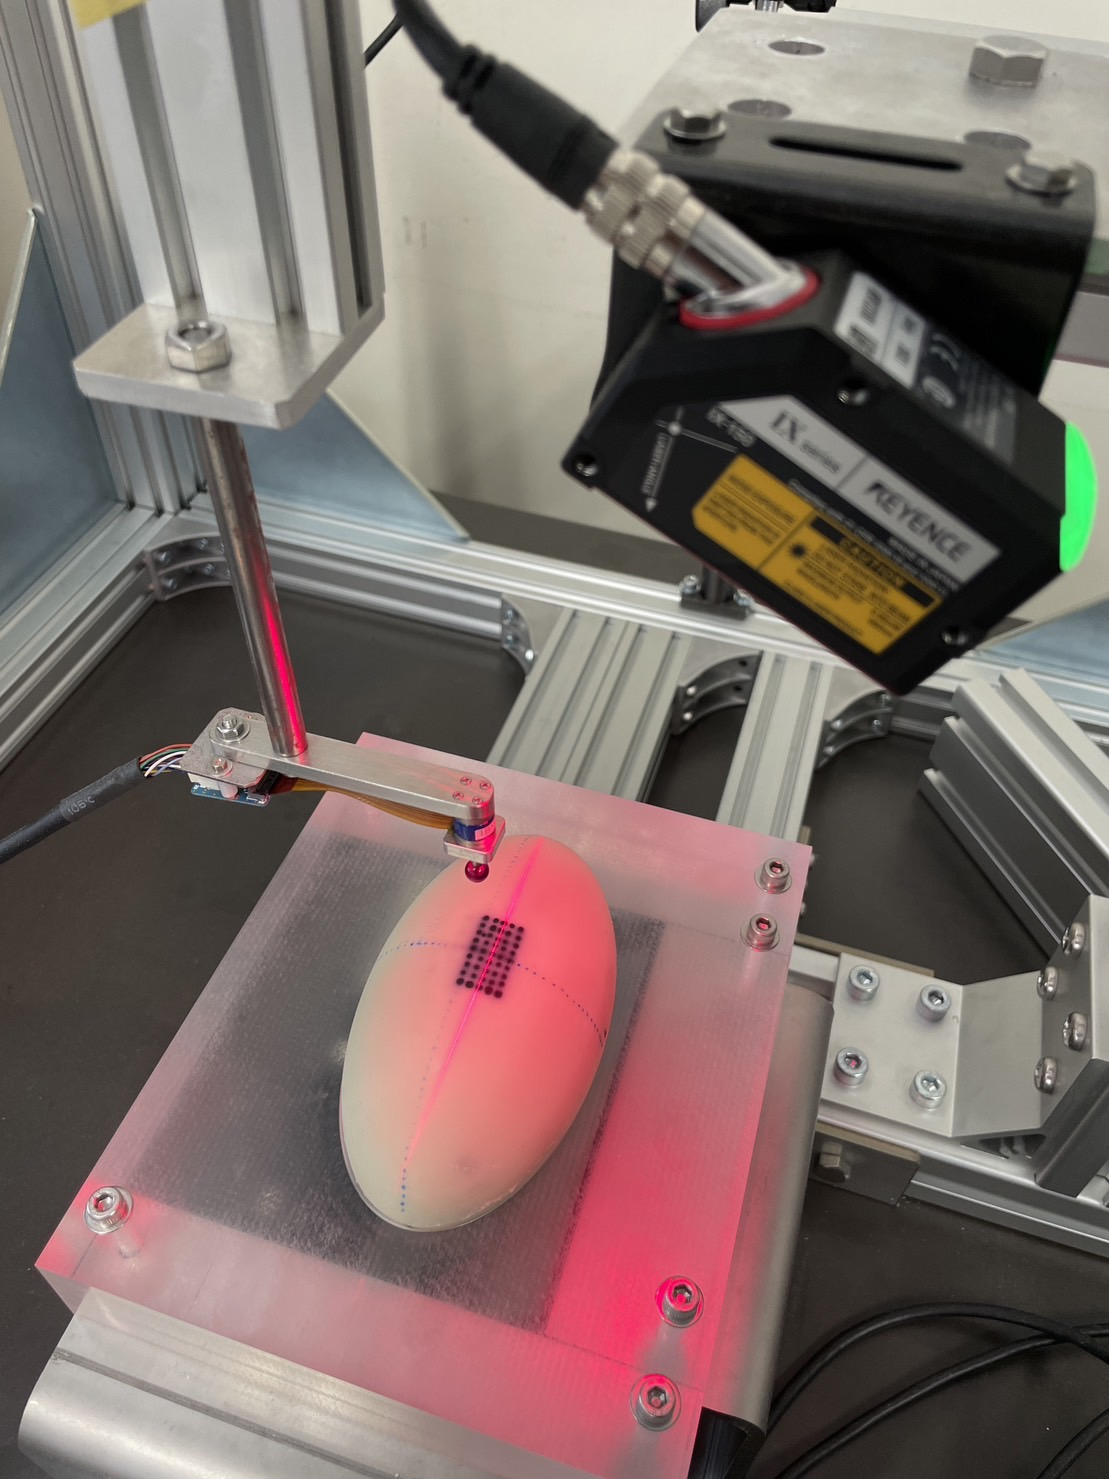
\includegraphics[width=6.5cm]{Images/Experiment/secondexp2.jpg}}}%
   \caption{YNU experimental model: 6-axis sensor Test Specimen made from ultra-soft polyurethane resin positioned on a fixed platform with a similar shape for constraint.}%
   \label{fig:secondexperiment}%
\end{figure}

\begin{figure}%
    \centering
   \quad
   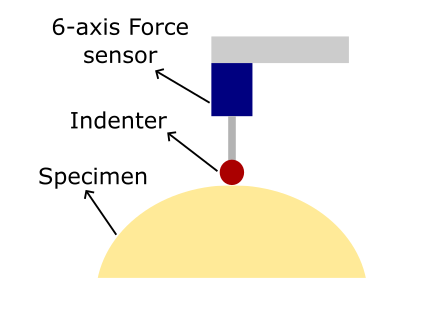
\includegraphics[width=6.5cm]{Images/Experiment/Loadingdiagram.png}%
   \caption{YNU experimental model: Loading diagram showing initial position of the indenter in normal position \cite{Mori2022}.}%
   \label{fig:loadingdiag}%
\end{figure}


The specimen, same as in the first experimental model (Section \ref{section:expmod1}),
 possessed the same dimensions, a minor radius $r_1 = \SI{35}{\milli \m}$ and a major 
 radius $r_2 = \SI{60}{\milli \m}$, and was
made from ultra-soft polyurethane resin. Consequently, the platform is also 
bowl-shaped. For this experiment, the platform base was made from transparent 
acrylic resin to record the contact status of the bottom surface \cite{Mori2022}. 
The maximum load capacity of the load cell is \SI{200}{\newton} and a theoretical 
force resolution of \SI{0.001}{\newton}. In addition, the resolution of the 
laser displacement sensor is \SI{0.05}{\milli \m}.
The indenter is sphere-shaped with a radius of $r_{i2} = \SI{3}{\milli \m}$ and
was made from ruby with the following specifications; 
a Young's Modulus of $E_{i2} = \SI{440}{\giga \pascal}$ and a Poisson's ratio of 
$\nu_{i2} = \SI{0.3}{\milli \m}$.

The indentation test was conducted under room temperature conditions. Also, 
the sample was placed on acrylic platform and the indenter was 
lowered at constant velocity of \SI[per-mode = symbol]{30}{\milli \m\per \minute}. 
The experiments were conducted for each loading point five times on the same sample, 
and the average of the results were calculated.

Furthermore, to minimize the friction during the indentation processs, the indenter 
and the loading surface on the specimen were covered with a thin layer of lotion. 
This was done due to inaccuracies shown in the measurements. Therefore, to reduce 
this measurement error, the application of lubricant was employed, ensuring a 
smoother and more controlled indentation process. Finally, the data 
was also processed and assessed using Excel.


\section{Experimental Tests Description}

\subsection{Middle Point}
The first use case for the indentation test was performed at the midpoint 
of the major and minor axis of the ellipsoid (Fig. \ref{fig:midpoint}). This point was selected 
to ensure that the indentation was normal to the surface, thereby avoiding 
the influence of potential shear forces which could influence the 
measurements.

\begin{figure}%
    \centering
   \quad
   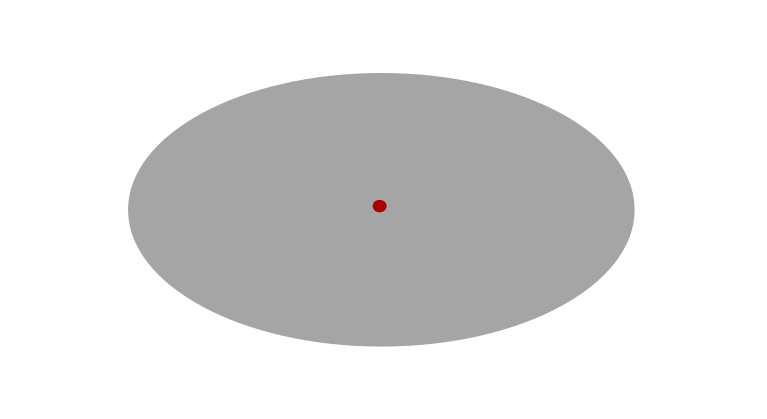
\includegraphics[width=6.5cm]{Images/Experiment/specimenmidp.png}%
   \caption{Middle test point: Loading point on the top surface of the specimen.}%
   \label{fig:midpoint}%
\end{figure}

Additionally, the first indentation depth was chosen arbitriarily, for the first 
experimental model was $h_{i1} = \SI{3.8}{\milli \m}$, and for the second 
experimental model was $h_{i2} = \SI{4}{\milli \m}$. This depth was considered 
to be an appropiate compromise that would allow to capture the nonlinear 
behavior of the material, while also remaining a simple use case to 
reproduce in a computational model in ANSYS.

As the main objective is to find a path, which lets identify the material 
 parameters, the most basic use case was selected and from this point 
the complexity was gradually built on. Through this approach, it was possible 
to establish a solid foundation for the subsequent experiments and data analysis.

\subsection{Load Unloading}
\subsection{Nearby Point}


\section{Analysis and Comparison of Experimental Techniques}

%write about the advantage and comparison
The second experimental model offers some advantages over the first model. 
Firstly, it enables not only the measurement of the total force reaction, but also the analysis 
of the force reaction components $F_x$, $F_y$ and $F_z$. This allows for a better 
understanding of the material's mechanical behavior, as it allows the identification 
of a specific contribution of the force components and it contributes to identify other 
mechanisms such as viscoelasticity, plasticity, and creep. 
In addition, the second model allowed for the measurement of the deformation in other 
points near the tested loading point. This provides additional information of the 
material parameters, as it facilitates the characterization of the deformation behavior beyond the 
direct vicinity of the indentation point.

In contrast, the first experimental model only measures the total force reaction 
against the indentation depth, without providing any information about the contribution 
of each component. While the first model allows the data 
gathering in simpler and more straightforward way, it may not capture 
the whole complexity of the material.

%For example, in a viscoelastic material, the initial loading response may be dominated by elastic behavior, followed by a time-dependent relaxation behavior as the material responds to the applied load. In contrast, a plastic material may exhibit a more gradual force response with continued loading, indicating the progressive deformation and flow of the material.
%By analyzing the force components during an indentation experiment, it is possible to separate out the contributions of different deformation mechanisms and gain a more nuanced understanding of the material's mechanical behavior. This can be achieved through various analytical techniques such as numerical simulations or mathematical models that take into account the material's constitutive behavior and mechanical properties.
%Overall, the observation of force components in an indentation experiment can provide important information about the underlying mechanisms contributing to the material's deformation behavior, which can be useful in a variety of engineering and scientific applications.


\subsection{Overview of the Data and Results}

Similar to the previous model, Fig. % add 
shows a nonlinear behavior with a maximum force reac

\subsection{Main Assumptions for Material Modeling}

For this project, there is a focus on the limitation of each material model, 
departing from an ideal scenario. From this point on the material will be build 
accordingly and for each model the influence of the material parameters is going
to be assessed.

\subsection{First Material model}

\subsubsection{Linear elasticity}


\subsubsection{Hyperelasticity}
The strain energy density function for the Neo-Hookean material model is given with
\begin{align*}
            \Psi = C_1 (I_1 - 3) \, ,
\end{align*}
where $C_1$ is a material constant and $I_!$ is the first invariant of the right Cauchy-Green tensor. 
Neo Hookean and Mooney Rivlin comparison

%Crear chart


% The approximated polynomial curve was used as a reference for the material modeling.

%test specimen is loaded at a quasi-static rate

% The measured force reation \(F_1\) data showed a very small number, so the 
% first 50 N load cell displayed a lot of noise in the measurements. 
% Therefore, the load cell was change to 10N to reduce this interference. 
%The 10 N load cell displayed the force-displacement curve of the indenter and the specimen
% in a finer way. 

%load unloading
Furthermore, in order to get the measurement of the load and 
 unloading process of
 the indentation a displacement sensor was attached to the tensile machine.

 The indentation depth \(h_1\) selected for the first model was 3,8 mm on the middle of the 
 top surface of the specimen. This indentation depth surpasses the pin radius \(r_3\) and 
 was chose arbitriarily to analyze the behavior of the material on the defined position.
 %reference?
 Additionally, it was observed that in soft materials it is easier to capture 
 some parameters with a larger indentation. Some references also observe that with
 indentation depth lower than indenter radius has a lot of noise and do not describe
 th results accurately. %reference?

 %results
 From the first experimental model we can observe that the material shows a nonlinear 
 behavior and the maximum total force reaction \(F_1\) lies around 0.45 N. %poner el grafico
 Furthermore, when applying different speeds, as show in Fig. %add figure 
 it is also possible to observe that 
 the hysteresis increases. %poner los speeds
This increasement shows that the material possesses a viscoelastic behavior, however
as this increasement is not significantly, it is possible to neglect viscoelasticity for 
the first stages of the project.

\begin{figure}[th]
    \centering
    \begin{tikzpicture}
        %\pgfplotsset{%legend outside the plot
        %every axis legend/.append style={ at={(1.05,0.95)}, anchor=north west,legend columns = 1}}
        \begin{axis}[
            %axis lines=middle,
            %x label style={at={(axis description cs:0.5,-0.1)},anchor=north},
            %y label style={at={(axis description cs:-0.1,.5)},rotate=90,anchor=south},
            xlabel={Displacement $u [mm]$},
            ylabel={Force reaction in Z-Axis $F_z [N]$},
            legend pos= north west]
            
            \addplot+[smooth, mark size = 1pt] table [y=$Force$, x=Def]{Table/data1.dat};
            %\addplot+[smooth] table [y=Force, x=$Def$]{Table/data2.dat};
            \legend{Experimental data}%,$l_2$}
        \end{axis}
    \end{tikzpicture}
    \caption[Expdata]{Experimental Load-displacement curve.}
    \label{fig:testgraph}
\end{figure}

